\chapter{Development of the Prototype}\label{chapter:development_prototype}



\section{Requirements}\label{section:requirements}

In order to provide the blockchain-based weather insurance, our system must fulfill several key requirements. In this section we describe each category of requirements in a dedicated subsection.

\subsection{Functional Requirements}

\begin{itemize}
    \item \textbf{Policyholder Interaction}
    \begin{itemize}
        \item The system must provide a user interface for purchasing policies and control information such as whether a payment has been triggered or the payment status. 
        \item This user interface should be kept with minimum need
    \end{itemize}


    \item \textbf{Weather Data Integration} 
    \begin{itemize}
        \item The system must be able to receive global weather data from reliable and trusted external sources such as Global Surface Summary of the Day (GSOD) and Global Forecast System (GFS)
        \item Both historical and forecast data must be available
    \end{itemize}
    
    
    \item \textbf{Smart Contract}
    \begin{itemize}
        \item The smart contract must allow users to purchase weather-based insurance policies.
        \item The smart contract must store the policy terms, including the weather conditions that will trigger an insurance payout.
        \item The contract must automatically trigger a payout when the predefined weather conditions are met.
    \end{itemize}
    
    \item \textbf{Oracle Integration}
    \begin{itemize}
        \item The system must use Chainlink oracles to retrieve and verify weather data from GCP datasets.
        \item Chainlink oracles must ensure secure transmission of data to the smart contract.
    \end{itemize}
    
    
    
    \item \textbf{Payout Processing}
    \begin{itemize}
        \item The system must automatically execute payouts without manual intervention when conditions are met.
    \end{itemize}
\end{itemize}

\subsection{Non-Functional Requirements}

\begin{enumerate}
    \item \textbf{Security}
    \begin{itemize}
        \item All interactions between the smart contract and Chainlink oracle must be secure.
        \item The system must protect the privacy of policyholder data.
    \end{itemize}
    
    \item \textbf{Reliability}
    \begin{itemize}
        \item The system must retrieve weather data consistently from reliable sources.
    \end{itemize}
    
    \item \textbf{Scalability}
    \begin{itemize}
        \item The system must scale to handle multiple policies and users.
    \end{itemize}
    
    \item \textbf{Transparency}
    \begin{itemize}
        \item All transactions and insurance claims must be recorded on the blockchain for transparency.
    \end{itemize}
    
    \item \textbf{Performance}
    \begin{itemize}
        \item The system must respond to data requests and process conditions efficiently.
    \end{itemize}
\end{enumerate}

\subsection{Technical Requirements}

\begin{enumerate}
    \item \textbf{Blockchain Platform}
    \begin{itemize}
        \item The system must be deployed on the Ethereum blockchain, supporting smart contracts in Solidity.
    \end{itemize}
    
    \item \textbf{Data API}
    \begin{itemize}
        \item The system must use APIs to retrieve weather data from GCP.
    \end{itemize}
    
    \item \textbf{Chainlink Oracle}
    \begin{itemize}
        \item The system must integrate with a Chainlink node to facilitate data retrieval from GCP.
    \end{itemize}
\end{enumerate}

\section{Inclusion of Chainlink and Google Cloud Public Datasets}\label{section:inclusion_chainlink_google_cloud_datasets}
\section{Designing the architecture and the data flow}\label{section:designing_architecture_data_flow}

\subsection{Architecture}

In \ref{fig:architecture} we present an overview of the general architecture that implements the requirements specified in \ref{section:requirements}. 

\begin{figure}[h]
    \centering
    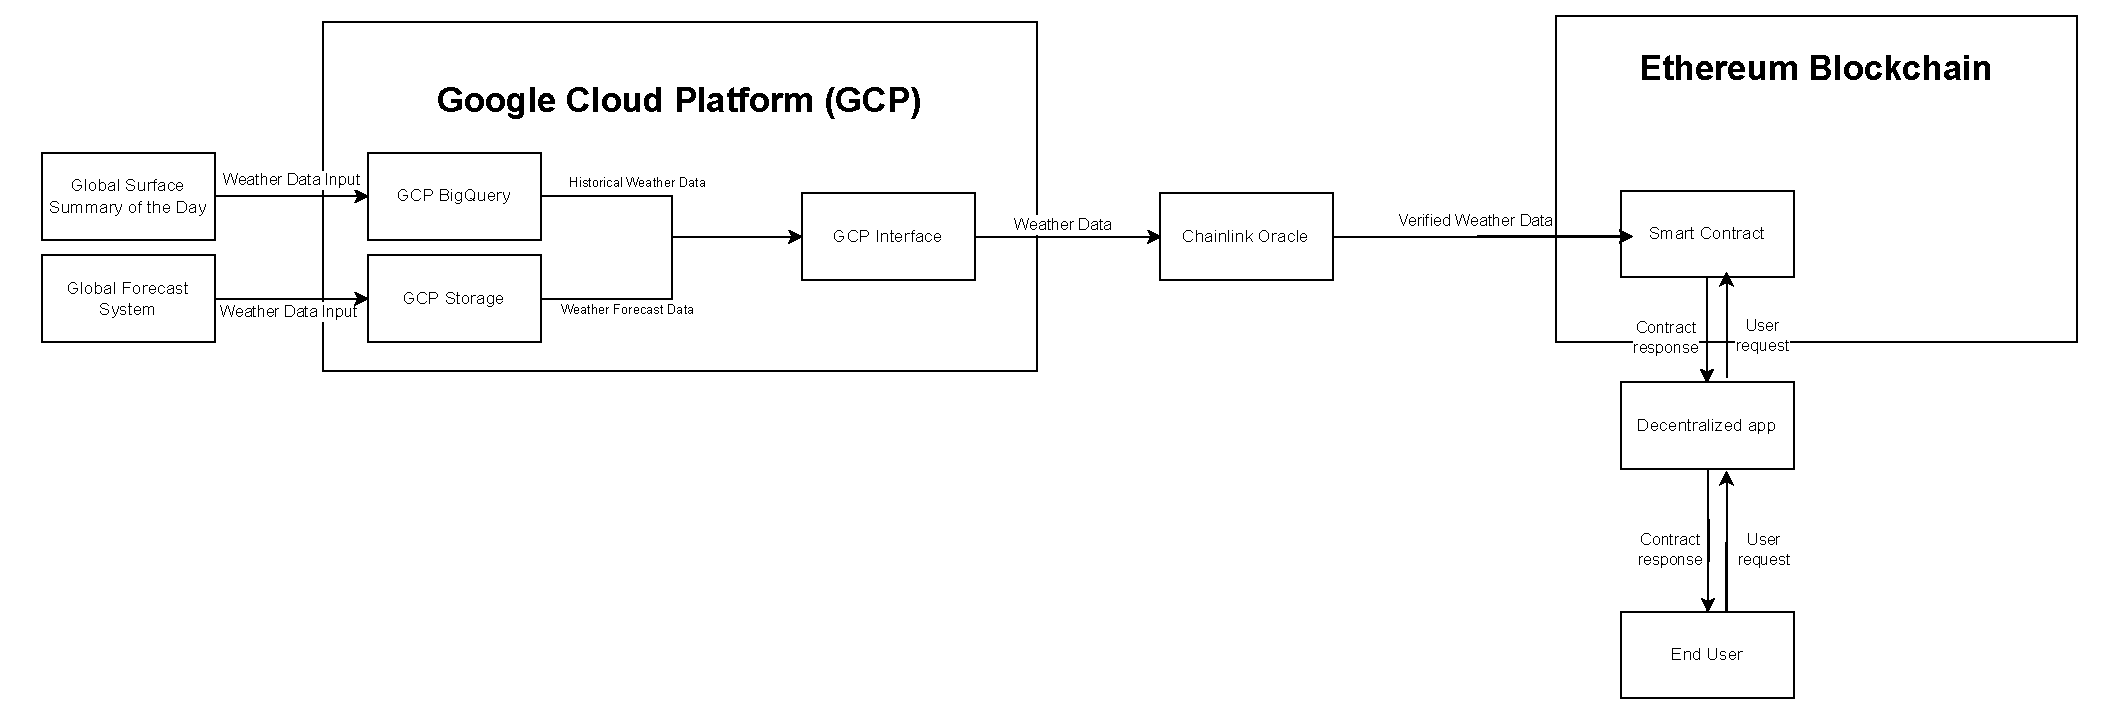
\includegraphics[width=0.8\textwidth]{figures/architecture-overview.drawio.pdf}
    \caption{Diagram showing the architecture of the smart contract}
    \label{fig:architecture}
\end{figure}